\documentclass{article}\usepackage[]{graphicx}\usepackage[]{color}
%% maxwidth is the original width if it is less than linewidth
%% otherwise use linewidth (to make sure the graphics do not exceed the margin)
\makeatletter
\def\maxwidth{ %
  \ifdim\Gin@nat@width>\linewidth
    \linewidth
  \else
    \Gin@nat@width
  \fi
}
\makeatother

\definecolor{fgcolor}{rgb}{0.345, 0.345, 0.345}
\newcommand{\hlnum}[1]{\textcolor[rgb]{0.686,0.059,0.569}{#1}}%
\newcommand{\hlstr}[1]{\textcolor[rgb]{0.192,0.494,0.8}{#1}}%
\newcommand{\hlcom}[1]{\textcolor[rgb]{0.678,0.584,0.686}{\textit{#1}}}%
\newcommand{\hlopt}[1]{\textcolor[rgb]{0,0,0}{#1}}%
\newcommand{\hlstd}[1]{\textcolor[rgb]{0.345,0.345,0.345}{#1}}%
\newcommand{\hlkwa}[1]{\textcolor[rgb]{0.161,0.373,0.58}{\textbf{#1}}}%
\newcommand{\hlkwb}[1]{\textcolor[rgb]{0.69,0.353,0.396}{#1}}%
\newcommand{\hlkwc}[1]{\textcolor[rgb]{0.333,0.667,0.333}{#1}}%
\newcommand{\hlkwd}[1]{\textcolor[rgb]{0.737,0.353,0.396}{\textbf{#1}}}%
\let\hlipl\hlkwb

\usepackage{framed}
\makeatletter
\newenvironment{kframe}{%
 \def\at@end@of@kframe{}%
 \ifinner\ifhmode%
  \def\at@end@of@kframe{\end{minipage}}%
  \begin{minipage}{\columnwidth}%
 \fi\fi%
 \def\FrameCommand##1{\hskip\@totalleftmargin \hskip-\fboxsep
 \colorbox{shadecolor}{##1}\hskip-\fboxsep
     % There is no \\@totalrightmargin, so:
     \hskip-\linewidth \hskip-\@totalleftmargin \hskip\columnwidth}%
 \MakeFramed {\advance\hsize-\width
   \@totalleftmargin\z@ \linewidth\hsize
   \@setminipage}}%
 {\par\unskip\endMakeFramed%
 \at@end@of@kframe}
\makeatother

\definecolor{shadecolor}{rgb}{.97, .97, .97}
\definecolor{messagecolor}{rgb}{0, 0, 0}
\definecolor{warningcolor}{rgb}{1, 0, 1}
\definecolor{errorcolor}{rgb}{1, 0, 0}
\newenvironment{knitrout}{}{} % an empty environment to be redefined in TeX

\usepackage{alltt}
\usepackage[normalem]{ulem}
\useunder{\uline}{\ul}{}
\usepackage{geometry}
\geometry{verbose,tmargin=1in,bmargin=1in,lmargin=1in,rmargin=1in}
\usepackage{fancyhdr}
\pagestyle{fancy}
\setlength{\parskip}{\smallskipamount}
\setlength{\parindent}{10pt}
\usepackage{amsthm}
\usepackage{algorithm,algorithmic,amsmath}
\usepackage{amsmath}
\usepackage[normalem]{ulem}
\useunder{\uline}{\ul}{}
\IfFileExists{upquote.sty}{\usepackage{upquote}}{}
\begin{document}

\title{Lab 4: Cloud Data \\ Stat 215A, Fall 2017}

\author{Jordan Prosky, Hongxu Ma, Alexander Brandt}

\maketitle 

\section*{Introduction}

In this lab we take a look at three different collections of spectroradiometric data from five satellite bound cameras relating to scenes of clouds near or in the arctic circle.  Cloud classification has long been an important task in geological and climate science.  Given the large volume of data generated by ever-improving satellite and aeroplane affixed instruments, labeling and identifying clouds in an automated fashion remains a challenge.  Our arctic datasets are particularly challenging, given that feature analysis algorithms from standard photographs is often confounded when presented with a similarity of feature and background color.  For scenes such as these, this means that the white of a cloud can often be confused with the white of a glacier or snow covered mountain.
Each camera samples light at four different light wavelengths.  And each of the five different camera was positioned at various angles and specified marked by a two letter code (DF, CF, BF, AF, or AN).  We have the following features for every pixel in our images:
\begin{itemize}
\item Local y coordinate
\item Local x coordinate
\item An manually labeled expert classification for cloud presence, absence, or ambiguity
\item Normalized Differential Angular Index (discussed more below)
\item The standard deviation of the zenith angle camera (discussed more below)
\item The radiance measurement at angle DF for red wavelength
\item The radiance measurement at angle CF for red wavelength
\item The radiance measurement at angle BF for red wavelength
\item The radiance measurement at angle AF for red wavelength
\item The radiance measurement at angle AN for red wavelength
\end{itemize}

\section{Exploratory data analysis}

Given that Normalized Differential Angular Index has the functional form:

\[ NDAI = \frac{I_1 - I_2}{I_1 + I_2} \]

Here, \(I_1\) represents the radiance sampled from the spectroradiometer in the Df orientation: 70.5 degrees from the zenith angle, and \(I_2\) represents the radiance sampled from the An orientation.  In effect, this measurement takes into account the dispersional difference in radiant intensity.  The various wavelengths of light sampled all fall within the visible range (with the exception of one near-IR band), roughly 200 nm - 900 nm.  So for the purposes of this discussion, let’s assume our intuition about how EM waves work in the visible spectrum is valid for the purposes of this lab.

However, this is where problems with the data become more readily apparent.  The MISR (Multi-angel SpectroRadiometer) measures in terms of power/distance\(^3\).  In SI convention, this is \(W/m^3\), though this can often vary from application to application.  To our knowledge, there should be no negative terms in this calculation, and thus the NDAI ratio should be bounded from -1 to 1.  In practice, however, the histogram has a large bulk of the data outside the expected range.

We will show below that the NDAI is still an excellent metric for classifying clouds vs. non-clouds, and it would be impossible to meaningfully complete this lab by throwing out values outside of the range show below in black bars (as it contains a vast majority of the pixels that were labeled by experts as clouds).  Computing our own NDAI values is also unfeasible, given that we lack the original intensities for the non-red colors measured by the satellite.  Nevertheless, this incongruity continues to be significantly concerning to the authors as they proceeded with their analyses, given that the measurements in question seem to have little correspondence with physical reality or the presented formula.

For the purposes of our discussion, we will assume some scaling factor was applied to NDAI, increasing the width, but not the character, of the underlying distribution.  See Figure 1.

We now turn our attention to Figure 2.  Here, anecdotally, we see that low NDAI correlates with non-cloud regions, and higher NDAI correlates with cloud or unlabeled regions.  This is because light in the visible spectrum will not be scattered preferential on incidence with the surface of the earth (especially on a white background, like the arctic images in our dataset).  This would imply an NDAI of around 0.  While we can’t be certain this fits with our data given the suspicious units, given the similarity to the histogram in Prof. Yu’s original paper and our own, we can hopefully assuming that we are off by a scaling factor.  This would suggest the taller constituent gaussian is centered closer \(NDAI = 0\), which fits with our physical intuition.

In contrast to the isotropically light scattered on the ground, incident light on the clouds in the visible spectrum scatters preferentially in the forward direction.  This leads to a much greater difference in our \(I_2\) and \(I_1\) terms, resulting in a larger NDAI.  Again, we can’t be sure what the exact NDAI we would expect from our data is, but given that it is more positive than the first constituent gaussian, it fits with our physical intuition.

It also explains why the SD column is such a useful metric, as it represents \(\sigma_{An}\), which is described in the paper as a quantification of the ground smoothness.  In fact, it is just the standard deviation of the true zenith angle spectroradiometer (the one which faces straight down from the satellite).  This is why lower confidence pixels, i.e., those with a higher SD, either track the outline of the cloud segments or show the clouds themselves.  The satellite attempts to take multiple measurements is sensitive because to objects varying spatially as a function of time.

To summarize, our radiances are not optimal for understanding the differences between cloud vs. non-cloud regions, almost certainly becasue they are only focused on the red wavelength.  NDAI, SD, and CORR are far better, given that they incorperate color multiple wavelengths, and/or multiple wavelengths over as function of neighbor proximity or variance.

\begin{figure}[h!]
\begin{center}
\caption{Troubling Histogram of NDAI}
\includegraphics[width = 0.4\textwidth]{figures/NDAI_Histogram.jpeg}
\end{center}
\end{figure}

\begin{figure}[h!]
\begin{center}
\caption{Spacial Distribution for the Expert Label, NDAI, and SD Values}
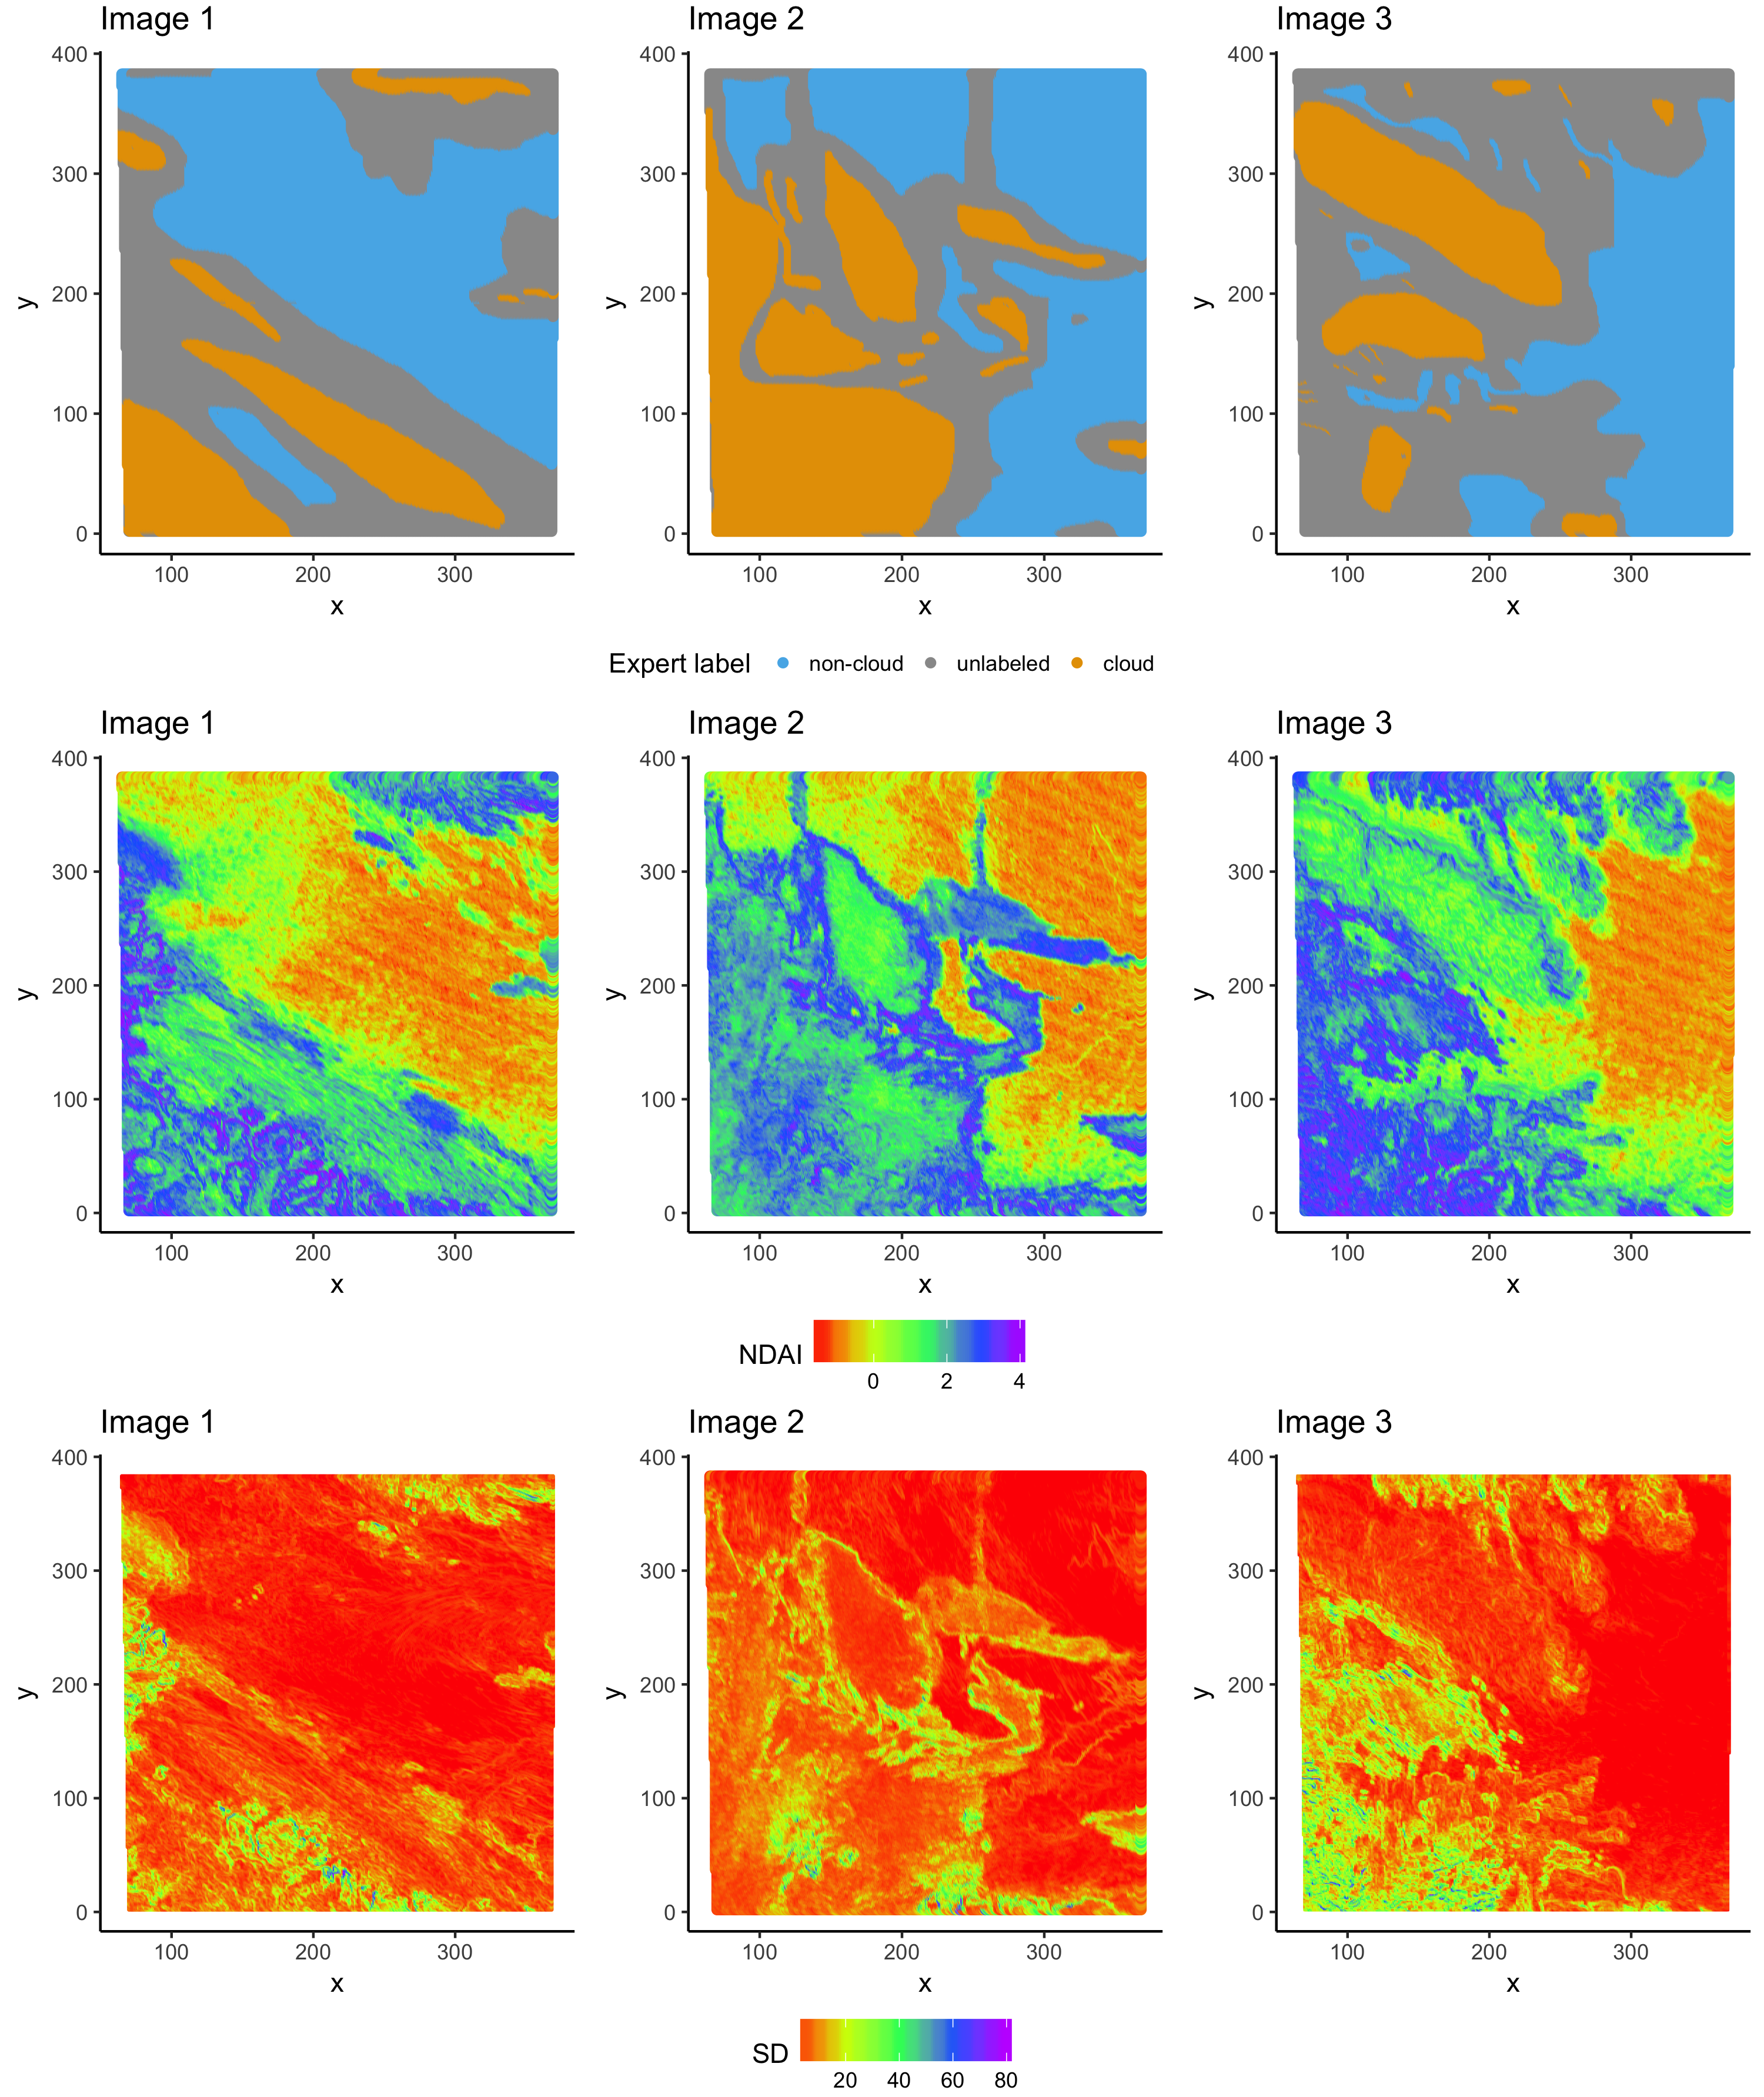
\includegraphics[width = 0.8\textwidth]{figures/EDA.png}
\end{center}
\end{figure}

\begin{figure}[h!]
\begin{center}
\caption{Class conditional densities for each feature}
\includegraphics[width = 0.8\textwidth]{figures/class_densities.pdf}
\end{center}
\end{figure}

\section{Modeling}

\subsection{Choosing the best predictors}

To abide by the principle of Occam's razor, it is desirable to select only 3 of
the 8 available features to use in our predictive modeling. Quick trial models
also support the idea that performance may be improved by performing clever
feature selection. Heuristically, the way that the NDAI, SD, and CORR features
were constructed by Shi et al. suggests that these features capture the information
present in the 5 individual radiance angle measurements. 

Quantitatively, we can begin by looking at the correlations between each feature
and the class label of each pixel. 

\begin{table}[h!]
\centering
\caption{Feature correlations with cloud presence}
\label{my-label}
\begin{tabular}{c|c|c|c|c|c|c|c|c|}
\cline{2-9}
                                       & \textbf{NDAI} & \textbf{SD} & \textbf{CORR} & \textbf{DF} & \textbf{CF} & \textbf{BF} & \textbf{AF} & \textbf{AN} \\ \hline
\multicolumn{1}{|c|}{\textbf{Image 1}} & 0.770         & 0.442       & 0.197         & -0.585      & -0.586      & -0.576      & -0.548      & -0.509      \\ \hline
\multicolumn{1}{|c|}{\textbf{Image 2}} & 0.819         & 0.474       & 0.750         & 0.309       & -0.253      & -0.515      & -0.584      & -0.573      \\ \hline
\multicolumn{1}{|c|}{\textbf{Image 3}} & 0.644         & 0.369       & 0.526         & 0.212       & 0.011       & -0.129      & -0.245      & -0.315      \\ \hline
\end{tabular}
\end{table}


While it is possible that the features may interact in a nonlinear
way to deternine whether a pixel has clouds or not, looking at the individual
linear correlations between features and cloud presence provides some valuable
insight. It is usually important to create models which 
are generalizable to out-of-sample data. We can think of each indvidiaul image as being out-of-sample
from the other two images, as they are taken from distinct regions. A model with good
generalization capabilities should take as input predictors which behave similarly
between in-sample and out-of-sample data. 
The high variability in correlations between the five radiance angle measurements
and class label suggest that these angle measurements may not be the most robust
features to be used in modeling if the goal is a model that can be used for more
than one image. On the contrary, the correlations between NDAI, SD, and COR are all
positive and similar in value (with the exception of CORR in image 1).

The feature densities in figure 3 of section 1 provide a clear visual guide to see which
features tend to separate classes well. Visually, the estimated densities for
NDAI and SD appear to be most split by class assignment. To pick a third feature,
we take note of the difference in tail behavior in the densities of CORR between
the classes. Further, we recall Shi et al. (2008) who used CORR values to make
decisions about class labels. This leads to our three features to be used for 
subsequent modeling: NDAI, SD, and COR. 

\subsection{Developing several 0-1 classifiers}

Using NDAI, SD, and CORR as features, we construct several 0-1 classifiers that
aim to predict whether a given pixel contains clouds or not. Aiming for a combination
of computational efficiency and model expressiveness, we chose to develop the following
four models: logistic regression (LR), quadratic discriminant analysis (QDA), 
random forest (RF), and a neural network (NN).

Each of the models makes various assumptions. The main ones are: 

\begin{itemize}
\item \textbf{LR}: Bernoulli response; linear relationship between features and log-odds; independent errors
\item \textbf{QDA}: multivariate normality of features
\item \textbf{RF}: bagging provides representative samples; nonlinear feature interaction
\item \textbf{NN}: cost function is differentiable; nonlinear feature interaction
\end{itemize}

Testing the assumption of linear or nonlinear feature interaction is an empirical question (measured by model performance), unless we are able to look at high-dimensional residual plots. 
Independence of errors in LR is quite hard to test, since errors are not directly observed.
The densities in section 1.2 support the multivariate normality of the features.
The one assumption that is difficult to justify is that bagging provides representative
samples in the RF model. The problem with some of the modeling techniques that use 
data from more than 1 image is that it may be possible to create bootstrap samples
that are not balanced with data from the different images. A heuristic to mitigate this problem
is looking at empirical and generalization performance, as well as using a large number 
of trees in order to reduce the model's variance. 

Each of the models (except QDA) has at least one hyper-parameter. Neural networks
and random forests in particular have many of which to tune. For the sake of time,
we focus on tuning the following hyperparameters in the model selection process:
\textbf{(LR)} - regularization parameter $\lambda$, \textbf{(NN)} - number of neurons in the
hidden layer, \textbf{(RF)} - number of trees.

\begin{table}[h!]
\centering
\caption{Accuracies of various models trained and tested on each image}
\begin{tabular}{llllll}
                                          &                                       &                                   & {\ul \textbf{}}                       & {\ul \textbf{TEST}}                   &                                       \\ \cline{2-6} 
\multicolumn{1}{l|}{}                     & \multicolumn{1}{l|}{{\ul }}           & \multicolumn{1}{l|}{{\ul }}       & \multicolumn{1}{l|}{\textbf{Image 1}} & \multicolumn{1}{l|}{\textbf{Image 2}} & \multicolumn{1}{l|}{\textbf{Image 3}} \\ \cline{2-6} 
\multicolumn{1}{l|}{}                     & \multicolumn{1}{l|}{\textbf{Image 1}} & \multicolumn{1}{l|}{\textit{LR}}  & \multicolumn{1}{l|}{0.9157}           & \multicolumn{1}{l|}{0.8341}           & \multicolumn{1}{l|}{0.7320}           \\ \cline{2-6} 
\multicolumn{1}{l|}{}                     & \multicolumn{1}{l|}{}                 & \multicolumn{1}{l|}{\textit{QDA}} & \multicolumn{1}{l|}{0.9219}           & \multicolumn{1}{l|}{0.8400}           & \multicolumn{1}{l|}{0.7450}           \\ \cline{2-6} 
\multicolumn{1}{l|}{}                     & \multicolumn{1}{l|}{}                 & \multicolumn{1}{l|}{\textit{RF}}  & \multicolumn{1}{l|}{\textbf{1.0000}}  & \multicolumn{1}{l|}{\textbf{0.8920}}  & \multicolumn{1}{l|}{\textbf{0.7719}}  \\ \cline{2-6} 
\multicolumn{1}{l|}{}                     & \multicolumn{1}{l|}{}                 & \multicolumn{1}{l|}{\textit{NN}}  & \multicolumn{1}{l|}{0.9430}           & \multicolumn{1}{l|}{0.8817}           & \multicolumn{1}{l|}{0.7583}           \\ \cline{2-6} 
\multicolumn{1}{l|}{}                     & \multicolumn{1}{l|}{\textbf{Image 2}} & \multicolumn{1}{l|}{}             & \multicolumn{1}{l|}{}                 & \multicolumn{1}{l|}{}                 & \multicolumn{1}{l|}{}                 \\ \cline{2-6} 
\multicolumn{1}{l|}{{\ul \textbf{TRAIN}}} & \multicolumn{1}{l|}{\textbf{}}        & \multicolumn{1}{l|}{\textit{LR}}  & \multicolumn{1}{l|}{0.8285}           & \multicolumn{1}{l|}{0.9598}           & \multicolumn{1}{l|}{0.8159}           \\ \cline{2-6} 
\multicolumn{1}{l|}{}                     & \multicolumn{1}{l|}{}                 & \multicolumn{1}{l|}{\textit{QDA}} & \multicolumn{1}{l|}{\textbf{0.9009}}  & \multicolumn{1}{l|}{0.9537}           & \multicolumn{1}{l|}{\textbf{0.8246}}  \\ \cline{2-6} 
\multicolumn{1}{l|}{}                     & \multicolumn{1}{l|}{}                 & \multicolumn{1}{l|}{\textit{RF}}  & \multicolumn{1}{l|}{0.7535}           & \multicolumn{1}{l|}{\textbf{1.0000}}  & \multicolumn{1}{l|}{0.8219}           \\ \cline{2-6} 
\multicolumn{1}{l|}{}                     & \multicolumn{1}{l|}{}                 & \multicolumn{1}{l|}{\textit{NN}}  & \multicolumn{1}{l|}{0.8265}           & \multicolumn{1}{l|}{0.9625}           & \multicolumn{1}{l|}{0.8200}           \\ \cline{2-6} 
\multicolumn{1}{l|}{}                     & \multicolumn{1}{l|}{\textbf{Image 3}} & \multicolumn{1}{l|}{}             & \multicolumn{1}{l|}{}                 & \multicolumn{1}{l|}{}                 & \multicolumn{1}{l|}{}                 \\ \cline{2-6} 
\multicolumn{1}{l|}{}                     & \multicolumn{1}{l|}{\textbf{}}        & \multicolumn{1}{l|}{\textit{LR}}  & \multicolumn{1}{l|}{0.8729}           & \multicolumn{1}{l|}{0.9451}           & \multicolumn{1}{l|}{0.8211}           \\ \cline{2-6} 
\multicolumn{1}{l|}{}                     & \multicolumn{1}{l|}{}                 & \multicolumn{1}{l|}{\textit{QDA}} & \multicolumn{1}{l|}{0.9017}           & \multicolumn{1}{l|}{\textbf{0.9453}}  & \multicolumn{1}{l|}{0.8200}           \\ \cline{2-6} 
\multicolumn{1}{l|}{}                     & \multicolumn{1}{l|}{}                 & \multicolumn{1}{l|}{\textit{RF}}  & \multicolumn{1}{l|}{0.7682}           & \multicolumn{1}{l|}{0.9255}           & \multicolumn{1}{l|}{\textbf{1.0000}}  \\ \cline{2-6} 
\multicolumn{1}{l|}{}                     & \multicolumn{1}{l|}{}                 & \multicolumn{1}{l|}{\textit{NN}}  & \multicolumn{1}{l|}{\textbf{0.9393}}  & \multicolumn{1}{l|}{0.8223}           & \multicolumn{1}{l|}{0.8635}           \\ \cline{2-6} 
\end{tabular}
\end{table}

For a quick implementation and to get a glance at both in- and out-of-sample performance of each of these models, we trained and test each model on each of the images. Table 2 below displays the results. Some things to note are that RFs are very easily able to overfit the training data, QDA is a competitive model, logistic regression consistently underperforms, and neural networks yield results which appear to provide a nice balance between over- and under-fitting. 

Before we can compare the four models, it is only fair to tune the hyper-parameters in the NN, RF, and LR models. Table 3 below shows the results of the naive hyper-parameter search. The search involves performing 5-fold cross-validation (CV) for each hyper-parameter specification. 

\begin{table}[h!]
\centering
\caption{Hyper-parameter tuning results}
\label{my-label}
\begin{tabular}{cccccc}
\multicolumn{1}{l}{\textbf{}}       & \multicolumn{1}{l}{\textbf{}}           &                                         & \textbf{\begin{tabular}[c]{@{}c@{}}Penalized \\ Logistic \\ Regression\end{tabular}} & \multicolumn{1}{l}{\textbf{}}           & \multicolumn{1}{l}{\textbf{}}           \\ \hline
\multicolumn{1}{|c|}{$\lambda$:}    & \multicolumn{1}{c|}{1 $\times 10^{-1}$} & \multicolumn{1}{c|}{1 $\times 10^{-2}$} & \multicolumn{1}{c|}{1 $\times 10^{-3}$}                                              & \multicolumn{1}{c|}{1 $\times 10^{-4}$} & \multicolumn{1}{c|}{1 $\times 10^{-5}$} \\ \hline
\multicolumn{1}{|c|}{CV score:}     & \multicolumn{1}{c|}{0.8222}             & \multicolumn{1}{c|}{0.8606}             & \multicolumn{1}{c|}{0.8625}                                                          & \multicolumn{1}{c|}{0.8626}             & \multicolumn{1}{c|}{\textbf{0.8627}}    \\ \hline
                                    & \multicolumn{1}{l}{}                    &                                         & \textbf{\begin{tabular}[c]{@{}c@{}}Neural \\ Network\end{tabular}}                   & \multicolumn{1}{l}{}                    & \multicolumn{1}{l}{}                    \\ \hline
\multicolumn{1}{|c|}{$n_{hidden}$:} & \multicolumn{1}{c|}{8}                  & \multicolumn{1}{c|}{16}                 & \multicolumn{1}{c|}{64}                                                              & \multicolumn{1}{c|}{128}                & \multicolumn{1}{c|}{512}                \\ \hline
\multicolumn{1}{|c|}{CV score:}     & \multicolumn{1}{c|}{0.8953}             & \multicolumn{1}{c|}{0.9017}             & \multicolumn{1}{c|}{0.9043}                                                          & \multicolumn{1}{c|}{\textbf{0.9044}}    & \multicolumn{1}{c|}{0.9043}             \\ \hline
                                    & \multicolumn{1}{l}{}                    & \multicolumn{1}{l}{}                    & \textbf{\begin{tabular}[c]{@{}c@{}}Random \\ Forest\end{tabular}}                    & \multicolumn{1}{l}{}                    & \multicolumn{1}{l}{}                    \\ \hline
\multicolumn{1}{|c|}{$n_{trees}$:}  & \multicolumn{1}{c|}{50}                 & \multicolumn{1}{c|}{100}                & \multicolumn{1}{c|}{150}                                                             & \multicolumn{1}{c|}{200}                & \multicolumn{1}{c|}{250}                \\ \hline
\multicolumn{1}{|c|}{CV score:}     & \multicolumn{1}{c|}{0.9029}             & \multicolumn{1}{c|}{0.9035}             & \multicolumn{1}{c|}{\textbf{0.9043}}                                                 & \multicolumn{1}{c|}{0.9043}             & \multicolumn{1}{c|}{0.9039}             \\ \hline
\end{tabular}
\end{table}

\subsection{Model selection with cross-validation}

There are various issues to consider when performing model selection for the cloud data. We wish to find a model which generalizes well and has stable performance, which can be measured using various metrics like a cross-validation (CV) score and the area under the ROC curve (AUC). Because the three images of data we have give different performances when looked at individually, we would like to make sure that our models are being trained and evaluated on data that provides a balanced-representation of each image in the training and test sets. Again, the goal of this scheme is to produce a model which is not biased towards one particular image and can perform well on predicting the presence of clouds in any pixel in any image that contains similar data. 

To perform CV on each of our models, we use k-folds that are constructed to conatin one $k^{th}$ of the data in each image in each of the folds. This method gives folds which contain a balanced representation of the different training images. 

The model selection proceeds by performing 10-fold CV with image-balanced folds for each of the four models. The output of this CV scheme is a single cross-validation score, which is the mean prediction score on each of ten left out folds, as well as the standard deviation of the fold scores. A "best" model should have the highest CV score with a reasonably low standard deviation. 
Table 4 below reports the CV scores and their margins of error for each of our four models.

\begin{table}[h!]
\centering
\caption{10-fold CV results}
\label{my-label}
\begin{tabular}{|c|c|c|c|c|}
\hline
                   & \textbf{LR}        & \textbf{QDA}       & \textbf{RF}        & \textbf{NN}                 \\ \hline
\textbf{CV Score:} & $0.8606 \pm 0.002$ & $0.8581 \pm 0.002$ & $0.9040 \pm 0.002$ & $\mathbf{0.9047 \pm 0.003}$ \\ \hline
\end{tabular}
\end{table}

Another way we can compare models is by analyzing the ROC curve associated with each
model's predictions, which display a curve describing the relationship between
sensitivity (true positive rate) and specificity (false positive rate). A typical
metric for model performance with ROC curves is the area under the curve (AUC).
We can compare the AUC for the predictions of various models and choose the best
model according to the highest AUC.

For the ROC curve analysis, we create train and test folds (80-20 split) which are both
image- and class-balanced. That is, we follow the same class balancing procedure described
previously, but we also create seperate subsplits for each class in order to ensure
that the train and test splits within each image are class-balanced. We train each of
our four tuned models on the same training set, and evaluate the AUC of the models on 
the same test set. All of the ROC curves exhibit very similar shape, so we exclude their plots
as they are redundant. Table 5 below displays the AUC scores for each of our models, along with the kappa score, sensitivity, and specificity for the predictions on the test set.

\begin{table}[h!]
\centering
\caption{ROC curve analysis}
\label{my-label}
\begin{tabular}{|l|l|l|l|l|}
\hline
\multicolumn{1}{|c|}{}                    & \multicolumn{1}{c|}{\textbf{LR}} & \multicolumn{1}{c|}{\textbf{QDA}} & \multicolumn{1}{c|}{\textbf{RF}}     & \multicolumn{1}{c|}{\textbf{NN}} \\ \hline
\multicolumn{1}{|c|}{\textbf{AUC Score:}} & \multicolumn{1}{c|}{0.9478}      & \multicolumn{1}{c|}{0.9467}       & \multicolumn{1}{c|}{\textbf{1.0000}} & \multicolumn{1}{c|}{0.9648}      \\ \hline
\textbf{Kappa:}                           & 0.7623                           & 0.7756                            & \textbf{0.8360}                      & 0.7604                           \\ \hline
\textbf{Sensitivity}                      & \textbf{0.9079}                  & 0.8383                            & 0.8675                               & 0.8106                           \\ \hline
\textbf{Specificity}                      & 0.8543                           & 0.9686                            & \textbf{1.0000}                      & 0.9905                           \\ \hline
\end{tabular}
\end{table}

Using the AUC score as a model selection criterion, we see that the RFachieves the best performance. Because we believe that the model selection done with cross-validation is more robust than the ROC curve comparisons, we choose to use the CV score to select the best model. Moreover, there is reason to believe that a random forest is very overfit to this particular dataset of 3 images. We conclude that since the neural network has the highest CV and it is our "best" model, and the rest of our analysis will focus on analyzing the neural network's predictions. 

\subsection{A neural network cloud detection model}

Figure 4 below shows the training and test loss (left) and accuracy (right) as a function of the number of epochs trained. We also display a ROC curve (bottom) for the neural network on the test set which was formed in the way described in section 2.3.

\begin{figure}[h!]
\caption{Neural network convergence and ROC curve for test data}
\includegraphics[width = \textwidth]{figures/converge.png}
\end{figure}

\subsection{Patterns in misclassification errors}
First, we analyze the difference of distributions between two types of error (false-positive and false-negative) pixels as shown in figure 5.  

\begin{figure}[h!]
\caption{Distribution of each feature for two types of errors}
\includegraphics[width = \textwidth]{figures/2typeserror.png}
\end{figure}

The false-positive are shown in blue and the false-negative are shown in red.
The similar distribution in all features is the major reason for misclassification.
By doing K-S test, the results also show the distributions are statistically similar to each other. The p-value of K-S test are all below 0.0001.

Then, we analyze the difference of distribution between correctly and incorrectly classified pixels (Figure 6). 

\begin{figure}[h!]
\caption{Distribution of each feature for correctly and incorrectly classified pixels}
\includegraphics[width = \textwidth]{figures/correctanalysis.png}
\end{figure}

The correctly and incorrectly classified pixels have statistical significant similar distributions for most features (all with p-value for K-S test less than 0.0001) besides NDAI (with p-value greater than 0.05 for K-S test). The majority error is ranged from 0 to 3 in NDAI.

Last, we plot the two types of error along with the images (Figures 7, 8, and 9).
\begin{figure}[h!]
\caption{Spacial distribution of two types of errors of image1}
\includegraphics[width = \textwidth]{figures/img1.png}
\end{figure}
\begin{figure}[h!]
\caption{Spacial distribution of two types of errors of image2}
\includegraphics[width = \textwidth]{figures/img2.png}
\end{figure}
\begin{figure}[h!]
\caption{Spacial distribution of two types of errors of image3}
\includegraphics[width = \textwidth]{figures/img3.png}
\end{figure}

The red pixels are false-positive, those non-clouds classified as clouds are plotted as blue pixels and represent the false-negatives, those clouds classified as non-clouds.  The textured profiles represent the AN red band.

Most errors are those with obvious spatial patterns. These errors are gathered within a certain region.  
The rest of the errors are those scattered with no certain spatial patterns. 
For the errors with certain spatial patterns, false-positive errors (shown in red) are much more concentrated than those false-negative errors (shown in blue). The false-negative errors have striped pattern, and the stripe lines are perpendicular to the motion of the clouds. I think this stripe pattern is caused by the shifting of cloud between the times taken from the different angles.
We believe the scattered errors could be resolved by adding the surrounding values (perhaps NDAI) as features.  The pixels surrounded by regions of high cloud probability should also be considered to have a high probability of being classified as a cloud.

\subsection{Generalizability}

The generalizability of our models was a great concern throughout the modeling entire process. The data available to us includes only 3 images of the more than 40 that were used in the original analysis of the full data set. This leads to the issue of our models overfitting to the those 3 images. The different out-of-sample performances (section 2.2) for each image leads us to believe that it is easy to overfit to a particular image.

Cross-validation was one method we used to investigate the issue of model generalization, but the issue of only using data from the 3 images remained. Aggregating the pixel-level data from all of the images provided better stability in out-of-sample predictions, but this is not enough for us to say that our models would perform comparably on other data. Given more time, another cross-validation scheme that could have been used to perhaps create a more robust model is creating grids within each image and using a set of grids as folds for CV. The idea is that each image contains a rich amount of geophysical diveristy, and subdiving the data into folds that are local in space could be a way to reduce our model's variance by way of data augmentation.

If the goal is a model that can detect the presence of clouds, as long as the out-of-sample features are similarly distributed, we would not except our model to fail miserably, but we are uncertain. Having more training data and developing a more robust CV-scheme would help resolve this uncertainty. If we are able to assume that out-of-sample data is more-or-less exchangeable with the data in this lab, we would believe that our model will generelize well. Moreover, depending on the preference of the scientist who uses this model, they may prefer to use a model that has higher specificity (NN, RF) or another which has higher sensitivity (LR). 

\section*{Conclusion}

In this lab we present an exploration of spectroradiometric data from clouds over the arctic.
We train several models in order to distinguish regions of clouds vs. non-clouds, ultimately
selecting a neural network model, and show its efficacy, accuracy,
and generalizability with respect to classification vs. expert labels.  We find that while 
certain specific conditions frustrate the classification, generally, cloud vs. non-clouds can be determined
from a mixture of NDAI, SD, and CORR labels from the data set, even if the individual 
camera angle red wavelength radiences are less useful.

\end{document}
